\documentclass[a4paper,11pt]{article}

\usepackage[utf8]{inputenc}
\usepackage[czech]{babel}
\usepackage[left=2cm,top=3cm,text={17cm,24cm}]{geometry}
\usepackage{graphicx}
\usepackage{listings}
\usepackage{url}

\title{ISA - Laboratorní cvičení č.5\\
{\bf\large Monitorování sítě}}

\author{Vysoké učení technické v Brně}
%Toto cviční připravil Libor Polčák s využitím textů Patrika Halfara a Martina
%Holkoviče.

\date{\url{https://github.com/nesfit/ISA/tree/master/monitoring}}

\begin{document}

{\let\newpage\relax\maketitle}

%\include{macro_lecture}
\section*{Cíl laboratorního cvičení}
\begin{itemize}
  \item seznámit se s nástroji pro správu sítě
  \item naučit se práci s nástrojem SSH a správu klíčů 
  \item naučit se pracovat s protokolem Syslog a nástrojem rsyslog
  \item konfiguraci nástrojů pro monitoring Icinga2
\end{itemize}

\section*{Pokyny}
\begin{itemize}
  \item Do zadání nepište, slouží pro další skupiny. PDF verzi zadání
  i šablony konfiguračních souborů lze najít v IS u předmětu ISA.
  
  \item Na konci laboratorního cvičení nezapomeňte na poslední bod,
  tj. na {\bf Ukončení práce v laboratoři}!
  
  \item Zapnete si počítače pod Windows prihlaste se jako užívatel \textbf{root} s heslem \textbf{root4lab}
  \item Zapnete si VirtualBox kde se nacházejí 3 virtuální počítače. Zkontrolujte zda jsou všechny počítače v předdefinovaném stavu init.
  \item Pro skrolování v konzoli (nejen) ve vituálních počítačích používejte
    \texttt{Shift} + \texttt{PgUp}/\texttt{PgDn}.
  
  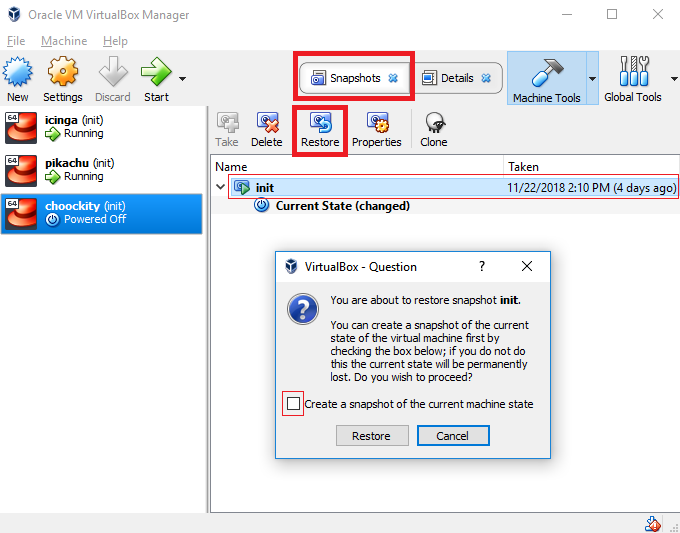
\includegraphics[width=\linewidth]{files/init.PNG}
  \item Všechny virtuální počítače mají 2 účty zapsané ve formě \textit{login/password}:
            \begin{itemize}
                \item \textbf{user/user4lab}
                \item \textbf{root/root4lab}
            \end{itemize}
\end{itemize}

\newpage
%\section{Laboratorní úlohy}
\section{Vzdálený terminál -- SSH}

Pracujte pod virtuálním počítačem pikachu a uživatelem {\tt user}. Zkontrolujte, že pracujete pod
uživatelem {\tt user} příkazem {\tt whoami}, který vypisuje jméno aktivního
uživatele.

Namísto řetězce {\tt <login>} používejte své studentské přihlašovací jméno.

\begin{enumerate}

  \item Pod uživatelem root ukončete démona spravujícího hesla k použitým klíčům SSH: 
  \begin{lstlisting}
  [user@pikachu]# su
  [root@pikachu]# pkill ssh-agent
  [root@pikachu]# exit
  \end{lstlisting}

  \item {\bf Bezpečné připojení na vzdálený počítač bez autentizačních klíčů.}

    \begin{enumerate}

      \item Přihlaste se příkazem {\tt ssh user@icinga} a zadejte heslo \textbf{user4lab}.

      \item Příkazem {\tt exit} nebo stiskem {\tt Ctrl-D} spojení ukončete.

    \end{enumerate}

  \item {\bf Vytvoření veřejného a privátního klíče.}

    \begin{enumerate}

      \item Příkazem {\tt ssh-keygen} vygenerujte implicitní klíč. Neměňte jeho
        název a zvolte heslo o délce alespoň osmi znaků například \textbf{pikapika}.

      \item Příkazem \verb|ssh-keygen -N "" -f ~/.ssh/nopass -C <login>@nopass| vygenerujte autentizační klíč bez hesla.

      \item Příkazem {\tt ssh-keygen -N <heslo> -f \textasciitilde/.ssh/pass -C
        <login>@pass} vygeneruje klíč s heslem jiným než pro výchozí klíč například \textbf{12345678}.

      \item Ověřte obsah a přístupová práva u nově vzniklých souborů (ls -l \textasciitilde/.ssh). Jak
se liší práva mezi souborem s privátním a veřejným klíčem?

    \end{enumerate}

  \item {\bf Distribuce klíčů}

    \begin{enumerate}

      \item Všechny tři veřejné klíče si zkopírujte na vzdálený počítač do
        souboru \verb|.ssh/authorized_keys|.
        (např. {\verb&ssh-copy-id -i <cesta k veřejnému klíči> <user>@<server>&}).
        
      Jaké heslo bylo nutné zadat?

      \item Zkuste se znovu přihlásit na stejný vzdálený počítač. Jaké heslo bylo nyní nutné zadat? Zkuste
zadat špatné heslo a pozorujte, které další klíče se použily. Při experimentech můžete také
využít tzv. verbose režim ssh ({\tt ssh -v}). Pro experimenty s identitou
využijte přepínač~{\tt -i}.

    \end{enumerate}

  \item {\bf Konfigurace použití klíčů}

    \begin{enumerate}

      \item Stejným způsobem nakopírujte své veřejné klíče ještě na další počítač \textbf{choockity}.

      \item Na svém počítači vytvořte soubor \textbf{\textasciitilde/.ssh/config} a pomocí textového editoru přidejte
        nasledující konfiguraci (hostname definujte jen pro jeden ze dvou strojů, na který jste
        kopírovali veřejné klíče):
        \begin{verbatim}
            Host icinga
                IdentityFile ~/.ssh/id_rsa

            Host *
                IdentityFile ~/.ssh/pass
                IdentityFile ~/.ssh/nopass
        \end{verbatim}
    \item Zmente prava v subore \textit{~/.ssh/config} pomoci príkazu:
      \begin{lstlisting}
        [user@pikachu]# chmod 600 ~/.ssh/config
      \end{lstlisting}
    
    \item Přihlaste se postupně na oba počítače. Které klíče se použily? Co se stane, když
pro některý klíč zadáte špatné heslo?

    \end{enumerate}

  \item {\bf Omezení použití klíčů}

    Nyní bude naším cílem omezit použití klíče, který není chráněn heslem tak,
    aby pomocí něj bylo možné na vzdáleném serveru vykonat pouze konkrétní příkaz.

    \begin{enumerate}

      \item Přihlaste se na počítač, kam jste nakopírovali své veřejné klíče a
        upravte soubor s autorizovanými veřejnými klíči tak, že na začátek
        řádku s klíčem nopass (řádek poznáte tak, že končí řetězcem
        {\tt <login>@nopass}) napíšete
        \verb|command="cat /etc/passwd" | (od původního
        obsahu oddělený jednou mezerou).

      \item Odhlaste se ze vzdáleného počítače icinga a znovu se na něj přihlaste
        příkazem {\tt ssh icinga -i \textasciitilde/.ssh/nopass}. Aplikovalo se
        omezené využití klíče?

    \end{enumerate}


  \item {\bf Pohodlné opakované použití klíče zabezpečeného heslem.}

    \begin{enumerate}

      \item Spusťte program ssh-agent:
      \begin{lstlisting}[language=bash]
            [user@pikachu]# eval $(ssh-agent -s)
      \end{lstlisting}

      \item Přidejte váš vygenerovaný klíč pomocí příkazu a zadejte heslo:
        \begin{lstlisting}[language=bash]
            [user@pikachu]# ssh-add ~/.ssh/id_rsa
            Enter passphrase for .ssh/id_rsa:
        \end{lstlisting}
      \item Přihlaste se k serveru icinga. Museli jste zadávat znovu heslo?
    \end{enumerate}
  \item Ověření konfigurace
    \begin{enumerate}
        \item Přihlaste se na počítač icinga (mělo by být možné bez hesla).
          Odhlašte se z počítače icinga.
        \item Na počítači pikachu použijte příkaz \textbf{ssh-add -d} a následně se opět přihlaste na 
        počítač icinga a stisknete 3-krát enter (měl by se vypsat obsah souboru /etc/passwd)
        \item Přihlaste se na počítač choockity a zadaje heslo 12345678
        \item Přihlaste se opět na počítač chockity, stisknete 2 krát enter.
    \end{enumerate}
  \item Pokud vám vše správně fungovalo vypnete počítač choockity, nebudeme ho v následujících úkolech potřebovat.

\end{enumerate}


\section{Syslog}
  \begin{itemize}
    \item Úkol: 
    \begin{itemize}
      \item Seznámit se s protokolem Syslog, který slouží pro přenos
      logovacích zpráv ze spravovaných zařízení. Pojmem Syslog je často označováno také
      programové vybavení implementující samotný přenos, třídění a ukládání zpráv na disk.
      \item Stanici \textbf{pikachu} si zvolte jako klient a \textbf{icinga} jako server a 
      nakonfigurujte přeposílání veškerých Syslog zpráv z klienta na server. Mějte na paměti 
      možné zneužití Syslog protokolu útočníkem a omezte na straně serveru příjem pouze na 
      zprávy od daného klienta a klientovi zamezte příjem jakýchkoliv zpráv ze sítě.
      \item Pro práci využijte nástroj {\tt rsyslogd}, který bude sloužit jako server i klient.
      K otestování využijte nástroj {\tt logger}.
      \item Na klientovi následně omezte přeposílání pouze na zprávy konkrétního typu.
      \item Na obou stanicích pracujte jako uživatel root.
    \end{itemize}
    \item Příkazy:
       \begin{itemize}
            \item {\tt rsyslogd(8)} -- démon pro Syslog.
            \item {\tt rsyslog.conf(5)} -- Popis konfigurace rsyslog démona.
            \item {\tt logger(1)} -- Nástroj pro generování Syslog zpráv.
            \item {\tt tcpdump(1)}
        \end{itemize}
    \item Postup:
       \begin{enumerate}
            \item {\bf Na serveru} povolte naslouchání na síťovém soketu. Do souboru {\tt /etc/rsyslog.conf} přidejte nebo odkomentujte:
\begin{verbatim}
  $ModLoad imudp
  $UDPServerRun 514
\end{verbatim}

            \item {\bf Na klientovi} zakažte programu rsyslogd naslouchat na síťovém soketu,
tj. odeberte/zakomentujte v souboru {\tt /etc/rsyslog.conf} řádky:
\begin{verbatim}
  $ModLoad imudp
  $UDPServerRun 514

  $ModLoad imtcp
  $InputTCPServerRun 514
\end{verbatim} 

            \item {\bf Na klientovi} nakonfigurujte rsyslog démona tak, aby odesílal veškeré zprávy
         z klienta na serveri pomocí UDP. Jako oddělovač použijte výhradně tabulátor nikoliv mezery.
         Do souboru {\tt /etc/rsyslog.conf} přidejte následující pravidlo:
\begin{verbatim} 
 *.*<TAB>@<doménové_jméno_serveru>:<číslo_portu>
\end{verbatim}

            \item {\bf Na serveru i klientovi} restartujte Syslog démona: 
\begin{verbatim}
  systemctl restart rsyslog
\end{verbatim} 

            \item {\bf Z klienta} ověřte správnou konfiguraci vygenerováním testovací Syslog 
         zprávy pomocí nástroje {\tt logger}:
\begin{verbatim} 
  logger -d <obsah_zprávy>
\end{verbatim} 
        
            \item Zpráva byla přeposlána na server, kde ji lze najít na konci souboru
         {\tt /var/log/messages}.

\begin{verbatim} 
  tail -f /var/log/messages | grep <doménové_jméno_klienta>
\end{verbatim} 

            \item  Na klientovi pokračujte v generování Syslog zpráv a 
         na serveru sledujte příchozí Syslog zprávy pomocí {\tt tcpdump}. Na jakém
         portu a jakým protokolem jsou Syslog zprávy zasílány.
         
         

            \item Otevřete si manuálovou stránku rsyslog.conf a zjistěte, jaké zařízení a priority
         zpráv Syslog poskytuje. FIXME konkretizovat
\begin{verbatim} 
  man rsyslog.conf
\end{verbatim} 
        
         \item Ze znalosti zařízení a priorit nakonfigurujte klienta, aby posílal na server 
         pouze zprávy při selhání autentizace, tj. upravte již existující pravidlo pro přeposílání
         veškerých zpráv na server v souboru {\tt /etc/rsyslog.conf}. Nezapomeňte restartovat Syslog démona. 
         
\begin{verbatim} 
  Syntax pravidel: <facility>.<priority><TAB><action>
\end{verbatim} 
         \item Ze serveru se následně pokuste o neúspěšné ssh připojení na klienta a podívejte se
         do souboru pro autentizační záznamy, jakou zprávu zaslal klient serveru.


       \end{enumerate}
   \end{itemize}

\section{Icinga2}
  \begin{itemize}
    \item Úkol: 
    \begin{itemize}
      \item Seznámit se s nástrojem Icinga2 pro monitorováni zařízení a servisů 
      \item Na klientské stanici nakonfigurovat nakonfigurovat kontroly služeb a
        živosti stanic.  
    \end{itemize}
    \item Poznámka:
        \begin{itemize}
            \item Na počítačích icinga a pikachu pracujeme pod uživatelem \textbf{root}
        \end{itemize}
    \item Postup:
       \begin{enumerate}   
            \item Ve Windows si otevřete webový prohlížeč a zadejte adresu 
            \textit{http://10.0.2.3}. Dostanete se na webové rozhraní Icingy2,
            která běží na počítači \textbf{icinga}.
               \begin{enumerate}
                   \item Přihlaste se pod uživatelem \textbf{user} a heslem \textbf{user4lab}
                    \item Přesměruje Vás to na rozhraní kde si můžete všimnout
                      monitoringu lokálních zařízení.
               \end{enumerate}
            \item Na zařízení icinga ve složce \textit{/etc/icinga2/conf.d} otevřete soubor \textbf{hosts.conf}, kde se nachází zakomentovaný příklad a do něj doplňte následující konfiguraci:
\begin{verbatim}
object Host "Pikachu" {
    address = "<PIKACHU IP ADDRESS>"
    check_command = "hostalive"
}

object Service "http" {
    max_check_attempts = 4
    check_interval = 10m
    retry_interval = 10m
    host_name = "<HOST NAME OF OBJECT>"
    check_command = "http"
}

\end{verbatim} 
            \item Restartujte službu
\begin{verbatim}
  systemctl restart icinga2.service
\end{verbatim} 
          \item Podívejte se na webové rozhraní Icingy2. Co se tam změnilo? 
          Když je nějaká služba down proč tomu tak je ?

          \item Na klientském počítací jménem pikachu zapnete webový server
\begin{verbatim}
  python -m SimpleHTTPServer <port>
\end{verbatim}
          \item Ve Webovém rozhraní Icingy2 v menu Overview|Services si
            vyhledejte předešlou kontrolu běžícího HTTP serveru. Pokud je služba
            ve stavu \emph{down}, klikněte na odkaz \textit{Check Now}. Změnilo se něco oproti předešlému stavu z bodu 4?

          \item Jaký je interval mezi jednotlivými kontrolami pro stanici
            Pikachu? Porovnejte tento interval s přednastaveními kontrolami.
            Jsou tyto intervaly rozdílné ? Pokud ano proč?

\end{enumerate}
\end{itemize}

\section*{Ukončení práce v laboratoři}
\begin{itemize}
  \item Vypněte všechny virtuální instance s aktivní možností obnovit na původní
    snímek \emph{init}.
          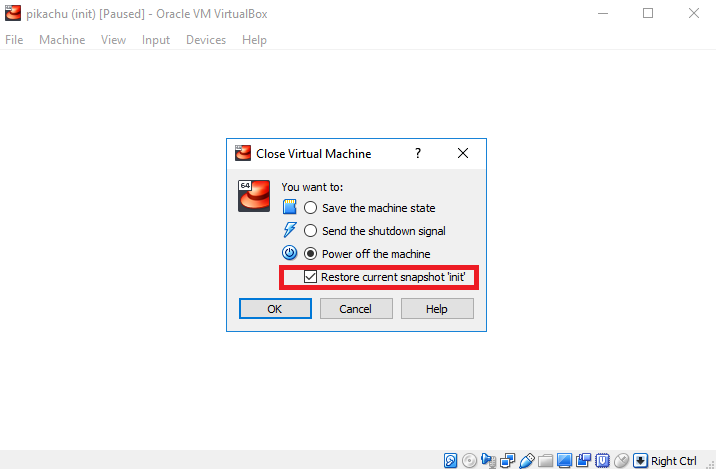
\includegraphics[width=\linewidth]{files/end.PNG}

\end{itemize}


\newpage
\setcounter{section}{0}
\section*{Teorie}

%%%%%%%%%%%%%%%%%%%%%%%%%%%%%%%%%%%%%%
\section{Network Time Protokol}
\label{ntp}
NTP \cite{rfc1305} umožňuje synchronizovat čas mezi uzly v~síti. Tento protokol se dokáže
vypořádat s~proměnlivou dobou přenášení paketu po síti. NTP organizuje servery hierarchicky do úrovní.
Tyto úrovně se nazývají {\em stratum}. Nejnižší hodnota 0 označuje samotný zdroj přesného času (např.
GPS). Stratum 1 pak označuje servery, které jsou synchronizovány právě s~referenčním zdrojem. Stratum 2
jsou servery synchronizovány se servery stratum 1, atd. \cite{rfc5905}.

Implementaci protokolu NTP zajišťuje balík aplikací {\em ntp}. Tento balík se skládá z~několika
aplikací. V~rámci laboratorního cvičení se použijí aplikace {\tt ntpd}, {\tt ntpq} a případně {\tt ntpdc}.

\subsection{ntpd}
NTPD je aplikace, která běží na pozadí a neustále provádí kontrolu času s~nastavenými servery a případně upravuje lokální čas. Úprava lokálního času se provádí úpravou rychlosti běhu lokálního času. Pokud je lokální čas pozadu, resp. se předbíhá, tak se {\em zrychlují}, resp. {\em zpomalují} systémové hodiny. Tento způsob úpravy času znamená, že pokud je čas odchýlen o~několik minut, bude nějakou dobu trvat, než dojde k~jeho srovnání. Na druhou stranu se tak zabrání skokové změně a navíc čas se nikdy neposune do minulosti. Pokud je lokální čas odchýlen o~více než 1000 sekund (necelých 17 minut) aplikace to vyhodnotí jako chybu a skončí. Pokud se tak stane, objeví se zpráva v~systémovém logu. Zda aplikace běží, lze zjistit například příkazem {\tt ntpq -p} (aplikace skončí s~hláškou {\em ntpq: read: Connection refused} pokud není ntpd spuštěn).

Démona je možné spustit příkazem:
\begin{verbatim}
systemctl start ntp.service
\end{verbatim}
Aby se předešlo problému v~případě, kdy např. hardwarové hodiny jdou špatně a při vypnutí může dojít k~odchýlení lokálního času o~více než 17 minut, je možné vynutit okamžité nastavení času příkazem
\begin{verbatim}
ntpd -qg
\end{verbatim}
({\tt -q} pro vynucení okamžitého nastavení času a {\tt -g} pro vypnutí kontroly kdy je rozdíl větší než 1000 sekund).

\subsubsection{Konfigurace}
Základním konfiguračním souborem je {\tt /etc/ntp.conf}. Tento konfigurační soubor obsahuje mnoho
konfiguračních voleb. Nastavení serverů NTP zajišťuje konfigurační volba {\em server}, která má jeden
parametr (adresu nebo jméno NTP serveru). Tato volba se může vyskytovat opakovaně, klient pak využívá
větší počet serverů a tím lze dosáhnout vyšší přesnosti. Volba server mimo jiné znamená, že lokální čas
se může nastavit podle uvedeného serveru, ale nemůže tomu být naopak. V~jiných případech může být volba
{\em server} nahrazena volbou {\em peer}, která umožňuje, aby se i server synchronizoval podle lokálních
hodin. Tato volba je užitečná, pokud je více ekvivalentních serverů, k~zajištění, že se budou
synchronizovat navzájem mezi sebou. Dalšími možnostmi jsou {\em broadcast} a {\em manycastclient}. Tyto
možnosti využívají broadcastového nebo skupinového vysílání (pokud je nutné synchronizovat velký počet
uzlů může tato možnost šetřit síťové zdroje). Server v~této konfiguraci vysílá na broadcastovou nebo
multicastovou adresu informace o~správném čase v~pravidelných intervalech a klienti zpracovávají tyto
informace.

Jinou užitečnou volbou je {\em restrict}, která slouží pro řízení přístupu. Aplikací {\tt ntpd} mohou být zaslány různé požadavky přes síť (viz aplikace {\tt ntpq}/{\tt ntpdc}). Je vhodné dovolit některé dotazy jen z~určitého uzlu nebo podsítě. Využití této volby může být také užitečné v~případě, že se pro nastavování času využívá broadcastu nebo multicastu a není žádoucí, aby takto vyslanou informaci klienti akceptovali z~libovolného zdroje. Základní tvar tohoto příkazu je:
\begin{verbatim}
restrict <adresa> [mask <maska>] [<jeden či více příznaků>]
\end{verbatim}

Příznak definuje omezení pro danou adresu/síť:
\begin{itemize}
  \item ignore -- zahazovat všechny pakety
  \item nomodify -- povolí pouze dotazy, požadavky měnící stav serveru jsou zahazovány
  \item noquery -- zakáže dotazy pomocí {\tt ntpq} a {\tt ntpdc}, synchronizace času není ovlivněna
  \item notrust -- zahazovat neautentizované pakety
\end{itemize}
Další příznaky a jejich popis lze nalézt v~manuálových stránkách {\tt man ntp.conf}.

Pokud budou aplikace {\tt ntpq} a {\tt ntpdc} používané i pro změnu konfigurace, pak je nezbytné nastavit autentizaci. Protokol nabízí možnost využití symetrické i asymetrické kryptografie. Pro použití symetrické kryptografie jsou k~dispozici tyto volby:
\begin{itemize}
  \item keys -- tato volba má jeden parametr, který udává název souboru, který obsahuje používané klíče (obvykle {\tt /etc/ntp.keys},
  \item trustedkey -- výčet klíčů, kterým se bude důvěřovat,
  \item requestkey -- seznam klíčů, které mohou být použity aplikací {\tt ntpdc},
  \item controlkey -- seznam klíčů, které mohou být použity aplikací {\tt ntpq}.
\end{itemize}
Formát souboru {\tt /etc/ntp.keys} má následující tvar:
\begin{verbatim}
<číslo klíče> <typ> <heslo>
\end{verbatim}
Typ může nabývat čtyř hodnot. Hodnoty {\tt S} a {\tt N} používají bitový formát a běžně se neužívají. Hodnoty {\tt A} a {\tt M} používají textový řetězce délky 1 až 8 znaků a určují způsob zašifrování při přenosu. Nejčastěji se užívá možnost {\tt M}, která značí použití DES nebo MD5. Příklad souboru pak může vypadat následovně:
\begin{verbatim}
1 M heslo1
2 M secret
3 M passwd
\end{verbatim}
Konfigurace v~{\tt /etc/ntp.conf} potom vypadá:
\begin{verbatim}
keys /etc/ntp.keys
trustedkey 1 2 3
requestkey 2
controlkey 1 3
\end{verbatim}
Toto značí, že důvěryhodné jsou všechny tři klíče. Aplikace {\tt ntpdc} se může autentizovat pouze klíčem 3 a aplikace {\tt ntpq} klíči 1 a 3.


\subsection{Aplikace ntpdc a ntpq}
Oba dva programy nabízejí v~podstatě podobné možnosti konfigurace ntp serveru. Rozdílů je mezi těmito programy několik. První, který byl již uveden výše, je v~tom, že každá z~těchto aplikací může používat jinou množinu klíčů. Podstatnější rozdíl z~uživatelského hlediska je v~tom, že aplikace {\tt ntpdc} má přesně definovaný výčet příkazů, které lze aplikovat, a proto může měnit jen to, co je v~aplikaci definováno. Naproti tomu {\tt ntpq} disponuje příkazem {\tt :config}, kterému se jako parametry předávají konfigurační volby, které se používají v~souboru {\tt /etc/ntp.conf}. Další rozdíl je ve formátu zpráv, pomocí kterých komunikují se serverem.

Obě aplikace používají pro komunikaci s~aplikaci {\tt ntpd} zasílání zpráv přes síťové rozhraní, bez ohledu na to, zda běží lokálně nebo vzdáleně. Hlavní výhoda však spočívá v~tom, že tyto aplikace dovolují měnit konfiguraci {\tt ntpd} za běhu. Možnost změny parametru přes síť může být nežádoucí a proto, je-li tato možnost povolena, je vhodné omezit pomocí volby {\em restrict} přístup pro změnu pouze přes loopback rozhraní.

Příklad výstupu volání {\tt ntpq -p}:

\begin{verbatim}
     remote           refid      st t when poll reach   delay   offset  jitter
==============================================================================
+rhino.cis.vutbr 248.205.243.78   3 u  425 1024  377   10.070   -4.280  10.575
+tik.cesnet.cz   195.113.144.238  2 u  622 1024  377    4.796   -3.464  16.528
*tak.cesnet.cz   .GPS.            1 u  364 1024  377    5.008   -3.625   6.228
\end{verbatim}

Výpis obsahuje následující hodnoty:

\begin{description}

  \item[remote] Klient se synchronizuje vůči třem serverům: rhino.cis.vutbr.cz,
    tik.cesnet.cz a tak.cesnet.cz. Hvězdičkou je označený primární zdroj času,
    plusem sekundární zdroje času.

  \item[refid] Primární zdroj času pro vzdálený server NTP.

  \item[stratum] Počet skoků od vzdáleného serveru k přesnému zdroji času (1
    znamená, že zdroj přesného času je přímo připojen, 16 znamená, že vzdálený
    server je nedosažitelný).

  \item[when] Počet sekund od posledního kontaktu se serverem.

  \item[poll] Počet sekund mezi jednotlivými dotazy protokolem NTP.

  \item[reachability] Úspěšnost posledním 8 pokusů o kontakt vzdáleného serveru
    v osmičkové soustavě. (1 znamená pouze poslední pokus uspěl, 377 znamená
    všech 8 posledních pokusů uspělo).

  \item[delay, offset, jitter] Zpoždění, posun a jitter -- charakteristiky
    vzdáleného zdroje času, podle kterého se volí primární a sekundární zdroje
    času.

\end{description}

%%%%%%%%%%%%%%%%%%%%
\section{Secure Shell}
\label{ssh}

Základní funkcí protokolu Secure Shell (SSH) \cite{rfc4253} je umožnění bezpečného přístupu ke vzdálenému počítači přes nezabezpečenou síť. Díky tomu, že je protokol SSH navržen
obecně, lze pomocí něj zabezpečovat i další služby, jako je např. X Windows, přístup ke vzdálenému souborovému systému (SFTP, sshfs, scp), tunelování portů TCP apod. Protokol SSH
zajišťuje šifrování dat, autentizaci, integritu dat a volitelně také kompresi přenášených dat.

V~rámci předmětu ISA se zaměříme pouze na malou část možností, které protokol SSH přináší. V~rámci cvičení si vyzkoušíme protokol SSH pro terminálový přístup ke vzdálenému stroji a
ukážeme si využití přihlašování ke vzdálenému počítači pomocí klíčů.

Jednou z~nejčastěji používaných aplikací pro využití protokolu SSH je sada programů OpenSSH. Balíček programů obsahuje kromě klienta {\tt ssh} i serverovou aplikaci {\tt sshd}, program
pro generování SSH klíčů {\tt ssh-keygen}, agenta pro usnadnění práce s~SSH klíči {\tt ssh-agent} a další. My budeme předpokládat, že na počítačích, na které se budeme snažit připojit
již běží SSH server {\tt sshd}. Konfigurace tohoto programu je nad rámec tohoto manuálu. Zájemci mohou nalézt podrobnější informace v~manuálové stránce {\tt sshd\_config(5)}, či
v~jiných návodech.

\subsection{Připojení ke~vzdálenému počítači}

Pro připojení se k~počítači pojmenovaném \emph{h01} a otevření příkazového řádku na vzdáleném stroji je možné použít příkaz:

\begin{verbatim}
ssh h01
\end{verbatim}

Příkaz ssh má celou řadu parametrů, které jsou detailně popsány v~manuálové stránce {\tt ssh(1)}. Z~těch nejčastěji používaných zmíníme alespoň změnu uživatelského jména ({\tt -l}),
specifikování TCP portu vzdáleného serveru ({\tt -p}), zvýšení výřečnosti programu ({\tt -v}, tento parametr lze použít i vícekrát), zapnutí tunelování protokolu X Windows ({\tt
-X}, {\tt -Y}) a přesměrování portů ({\tt -L}). Často zadávané parametry se specifikují v konfiguračním souboru \verb|~/.ssh/config|. Popis tohoto souboru obsahuje manuálová
stránka {\tt ssh\_config(5)}.

Po připojení ke vzdálenému serveru jsou informace o~použitém spojení dostupné např. v~rámci proměnných prostředí. Proměnné prostředí související s~protokolem SSH je možné zobrazit
příkazem {\tt env | grep SSH}. Následující výpis ukazuje příklad proměnných po připojí k~serveru {\tt merlin} protokolem IPv6:

\begin{verbatim}
local $ ssh merlin6.fit.vutbr.cz 
merlin $ env | grep SSH
SSH_CLIENT=2001:67c:1220:80c:e138:4d11:c04c:c675 54514 22
SSH_TTY=/dev/pts/30
SSH_CONNECTION=2001:67c:1220:80c:e138:4d11:c04c:c675 54514 2001:67c:1220:8b0::93e5:b013 22
\end{verbatim}

Z~výpisu vidíme, že připojení bylo realizováno na IPv6 adresu 2001:67c:1220:8b0::93e5:b013 z~počítače s~adresou 2001:67c:1220:80c:e138:4d11:c04c:c675. Byl použit zdrojový port č.
54514, na straně serveru byl použit standardní protokol 22. Po připojení využíval vzdálený uživatel terminál č. 30. Odhlášení ze vzdáleného počítače probíhá standardními
prostředky pro ukončení shellu, např. příkaz {\tt exit}, nebo vložení konce souboru klávesovou zkratkou {\tt Ctrl + D}.

\subsection{Kopírování souborů mezi počítači}

Pro kopírování souborů protokolem SSH je často využívaná utilita {\tt scp}. Cesta na vzdáleném serveru je specifikována v~následujícím formátu: uživatel@jménoserveru:cesta.
Následující příkaz zkopíruje lokální soubor isa na vzdálený počítač h01 do složky fit umístěné v~domovské složce uživatele student.

\begin{verbatim}
scp isa student@h01:fit/
\end{verbatim}

\subsection{Klíče protokolu SSH}

Klíče protokolu SSH mají několik výhod. Díky nim není nutné posílat heslo pro přístup ke vzdálenému stroji přes síť, byť v~šifrované podobě. Délka používaných klíčů znesnadňuje
potenciálnímu útočníkovi útok hrubou silou, protože síla klíče bývá typicky vyšší než síla běžně používaných hesel. Ve spojení s~agentem pro správu klíče může uživatel přistupovat ke
vzdálenému serveru bez nutnosti opakovaného zadávání hesla. Agent může být nastaven, aby pro použitý klíč nevyžadoval heslo po zbytek sezení, či po určitý počet minut.

SSH klíč se obvykle generují utilitou {\tt ssh-keygen}. Po spuštění bez parametrů je vytvořen pár klíčů algoritmem RSA o~délce 2048\,B. Uživateli je nabídnuto umístění souboru,
které může změnit. Dále je uživatel požádán o~zadání passfráze, od které se očekává, že bude silnější než heslo. Parametr {\tt -t} nastavuje jiný typ šifrovacího
algoritmu, parametr {\tt -b} mění délku klíče, parametrem {\tt -f} specifikuje umístění souboru, parametr {\tt -C} upravuje popis klíče, další
parametry popisuje manuálová stránka {\tt ssh-keygen(1)}. Následující příklad vygeneruje klíč o~délce 4096\,B, který nebude chráněn passfrázi:

\begin{verbatim}
ssh-keygen -t rsa -b 4096 -N "" -f ~/.ssh/nopass -C nopass
\end{verbatim}

Po vytvoření klíčů vzniknou dva soubory. Ten který je bez přípony {\tt .pub} je soukromý klíč, který by měl zůstat tajný a uživatel, který jej vytvořil by jej neměl dále distribuovat.
Soubor s~příponou {\tt .pub} je určen pro další distribuci, protože data zašifrovaná tímto klíčem dešifruje pouze tajný soukromý klíč.

\subsection{Konfigurace použití klíčů}

Nejdříve je potřeba distribuovat soubor s~veřejným klíčem na vzdálený počítač. K~tomu slouží např. program {\tt scp}. Každý z~uživatelů si může specifikovat sadu klíčů pro
přístup k~danému stroji v~souboru \verb|~/.ssh/authorized_keys|. Nový klíč do tohoto souboru přidáme např. takto (všimněte si, že se klíč přidává na konec souboru
pomocí \verb|>>|):

\begin{verbatim}
cat id_rsa.pub >> ~/.ssh/authorized_keys
\end{verbatim}

Nyní se již můžeme připojit ke vzdálenému počítači pomocí vytvořených klíčů. Pokud jsme klíč na lokálním počítači umístili do výchozího umístění, je klíč použit automaticky. Pokud jsme
zvolili jiné umístění, je potřeba program {\tt ssh} informovat o~umístění klíče parametrem {\tt -i}, nebo volbou {\tt IdentityFile} v~konfiguračním souboru. Informace o hledaných
klíčích jsou zobrazeny po použití parametru {\tt -v}.


%%%%%%%%%%%%%%%%%%%%%%%%%%%%%%%%%%%%%%
\section{Domain Name System}
\label{dns}
Cílem DNS je zajistit překlad mezi doménovým jménem a IP adresou. Dříve se jednalo především o~překlad hostname na IP adresu a naopak, tedy záznamy typu {\tt A}, {\tt AAAA}, {\tt PTR} \cite{rfc1035,rfc3596}. Dalším známým typem je {\tt MX}, který deleguje zodpovědnost za příjem e-mailové pošty dané domény. Tento typ se od předchozích tří odlišuje, protože se nejedná o~adresaci hosta, ale služby. Podobný význam mají i záznamy typu {\tt SRV}, které lze v~současnosti využít pro služby SIP a XMPP \cite{rfc2782}.

Mimo tyto typy záznamů existují i další. Některé jsou definovány již v~původním návrhu, jiné přidané později nebo význam původních typů vyžit pro další služby (např. {\tt TXT} využito pro distribuci veřejného klíče podepisování emailu DKIM \cite{rfc4871}).

\subsection{Klient}
Aby klient věděl, na který server se obrátit s~požadavkem na přeložení doménového jména na IP adresu či opačně, je součástí systému tzv. resolver. Tento resolver má několik konfiguračních souborů, z~nichž jmenujme {\tt /etc/hosts}, {\tt /etc/resolv.conf} a {\tt /etc/host.conf}.

První z~těchto souborů se používá pro statický překlad doménového jména na IP adresu. Formát souboru a další popis lze nalézt v~manuálových stránkách {\tt man hosts}.

Dynamický překlad, neboli překlad pomocí DNS serveru, vyžaduje existenci konfiguračního souboru {\tt /etc/resolv.conf}, který obvykle obsahuje jedenkrát volbu {\tt search} a jednu nebo více voleb {\tt nameserver}.
\begin{description}
  \item[search] definuje tzv. searchlist, neboli seznam domén (max. 6), které se budou prohledávat, pokud je požadavek na překlad neúplného doménového jména. Tedy má-li tato volba podobu {\tt search fit.vutbr.cz}, pak při pokusu přeložit jméno {\em merlin} se při neúspěchu pokusí systém také přeložit jméno {\em merlin.fit.vutbr.cz}.
  \item[nameserver] se uvádí právě s~jedním parametrem, který definuje IP adresu DNS serveru, který se systém pokusí kontaktovat. Může se jednat jak o~IPv4 tak o~IPv6 adresu.
\end{description}
Další možnosti, které může soubor obsahovat, lze nalézt v~manuálových stránkách {\tt man resolv.conf}.

V~souboru {\tt /etc/host.conf} lze definovat, v~jakém pořadí se předchozí dvě volby využijí. Standardně se nejprve zkouší statický překlad a poté dynamický. Toto výchozí nastavení umožňuje lokální předefinování překladu z doménového jména na IP adresu.

Pokud se síť na klientovi konfiguruje dynamicky, pak je soubor {\tt /etc/resolv.conf} upravován automaticky. Při statické konfiguraci musí být obsah souboru upraven ručně.

\subsection{Konfigurace serveru}
Konfigurace DNS se stává ze dvou částí -- konfigurace vlastností samotné aplikace a konfigurace obsluhovaných zón. Existuje mnoho různých variant implementací. V~laboratoři se bude pracovat s~implementací od ISC -- BIND.

Konfigurační soubor {\tt\bf named.conf} se na počítačích v~laboratořích nachází ve složce {\tt
/etc/bind/}. V Linuxové distribuci Kali tento soubor obsahuje vložené 3 soubory (pro konfiguraci voleb,
konfiguraci lokálních zón a konfiguraci výchozích zón).

%\begin{verbatim}
%
%acl "local" {
%  <prefix>/<délka prefixu>;
%};
%
%options {
%  listen-on-v6 { <ipv6 adresa lokálního rozhraní>; };
%  allow-query { local; };
%  allow-recursion { local; };
%  allow-transfer { none; };
%  allow-update { none; };
%  directory "/etc/namedb/working";
%  pid-file "/var/run/named/pid";
%}
%
%zone "." IN {
%  type hint;
%  file "/etc/namedb/named.root";
%};
%
%zone "localhost" IN {
%  type master;
%  file "/etc/namedb/master/localhost-forward.db";
%  notify no;
%};
%
%zone "127.in-addr.arpa" IN {
%  type master;
%  file "/etc/namedb/master/localhost-reverse.db";
%  notify no;
%};
%
%zone "0.ip6.arpa" IN {
%  type master;
%  file "/etc/namedb/master/localhost-reverse.db";
%  notify no;
%};
%
%zone "255.in-addr.arpa" IN {
%  type master;
%  file "/etc/namedb/master/empty.db";
%  notify no;
%};
%
%zone "0.in-addr.arpa" IN {
%  type master;
%  file "/etc/namedb/master/empty.db";
%  notify no;
%};
%
%\end{verbatim}

%Zóna typu {\tt hint} odkazuje na seznam tzv. root serverů, tedy takových serverů, které znají informace
%o všech registrovaných top-level doménách a dokáží říci, které servery jsou za tyto top-level domény
%zodpovědné. Zóna typu {\tt master} značí, že server je autoritativním serverem pro danou doménu.
%Mezi povinné záznamy pro takovou doménu patří záznam typu SOA a alespoň jeden NS odkazující na server samotný. Zároveň by měl být obsažen i záznam typu A pro tento server.
Další možnosti konfiguračního souboru naleznete v~manuálových stránkách {\tt man named.conf}.

\subsubsection{Zóna typu hint}
Asociuje se s~nejvyšší doménou v~rámci celé hierarchie. Pokud přijde na server požadavek, prohledá seznam spravovaných zón ostatních typů ({\em master}, {\em slave}, {\em forward}). Pokud záznam nenajde, vybere jeden z~kořenových serverů definovaný právě v~tomto typu zóny.

Soubor, který je vyžadován pro konfiguraci této domény lze získat například programem dig:
\begin{verbatim}
 dig +norec NS . @a.root-servers.net > /etc/bind/db.root
\end{verbatim}

\subsubsection{Lokálně obsluhovane zóny}
Tyto zóny lze rozdělit do dvou skupin -- {\bf loopback adresy} a {\bf ,,prázdné zóny''}. RFC 6303
\cite{rfc6303} je z~kategorie {\em best practice} a definuje, které zóny by měl být schopen DNS server
obsloužit sám a tím redukovat dotazy přeposílané na další servery. Ve většině případů jsou to zóny pro reverzní záznamy privátních IP adres.

%Výchozí soubor aplikace {\bf named} ve FreeBSD respektuje právě RFC 6303 a navíc doplňuje ještě další
%zóny. Například nealokované rozsahy IPv6 adres. Pro práci v~laboratoři nahraďte původní soubor {\tt
%/etc/namedb/named.conf} souborem {\tt /root/isa1/named.conf}, který je zkrácen a obsahuje pouze nezbytné definice.

\subsubsection{Vlastní zóna}
Aby server začal překládat vlastní zónu, je třeba přidat definici zóny do souboru {\tt named.conf.local} a vytvořit zónový soubor. Pokud se přidává zónový soubor pro doménu, je vhodné přidat i zónu pro reverzní záznamy.

\begin{verbatim}
zone "moje.domena.cz" {
  type master;
  file "/var/cache/bind/moje.domena.cz.zone";
};

zone "0.168.192.in-addr.arpa" {
  type master;
  file "/etc/bind/master/192.168.0.rev";
};
\end{verbatim}

Pro každou z~těchto zón se tvoří samostatný zónový soubor, jehož základní tvar má podobu:

%$ORIGIN <nazev domény>
\begin{verbatim}
%$TTL 5m

@ IN  SOA <fqdn autoritativniho serveru>. <email správce>. (
  1   ; seriové číslo
  10h ; obnovovací interval pro sekundární servery
  10m ; prodleva, po které se sekundární server pokusí znova kontaktovat
      ; autoritativní server, pokud se předchozi spojení nezdařilo
  1w  ; jestliže se sekundárnímu serveru nepodaří kontaktovat autoritativní
      ; server během této doby, přestane vracet záznamy pro tuto doménu
  1h  ; původně výchozí TTL (nahrazeno $TTL), nově určuje
      ; NEGATIVNÍ TTL -- pro chybové odpovědi (např. NXDOMAIN)
  )

@ IN  NS <fqdn autoritativního serveru>
@ IN  NS <fqdn sekundárního serveru>

následuje seznam dalších záznamů
\end{verbatim}
Typ záznamu {\tt\bf SOA} definuje parametry zóny -- jméno autoritativního serveru a email správce domény. Všimněte si, že znak `{\tt @}' má zvláštní význam (zastupuje název domény). Z~tohoto důvodu se v~emailu správce nahrazuje znak `{\tt @}' za znak `{\tt .}' (tečka).

Záznam typu {\tt\bf NS} by měl být vždy obsažen alespoň jednou a to právě pro autoritativní server. Počet sekundárních serverů je libovolný. Tyto záznamy by také měly byt obsaženy v~nadřazené doméně, aby bylo možné nalézt server zodpovědný za danou poddoménu. Tedy kořenová doména obsahuje {\tt NS} záznamy pro domény nejvyšší úrovně {\em .cz, .com, .eu, \dots} a ty zase pro jednotlivé poddomény {\em google.com, seznam.cz, \dots}.

V~zónovém souboru se rozlišuje mezi relativním a absolutním jménem. O~jaký typ jména jde, se rozlišuje podle zakončení. Končí-li tečkou, je to jméno absolutní (plně kvalifikované). V~opačném případě jde o~jméno relativní a za to se vždy doplní obsah definován v~{\tt \$ORIGIN}. Jestliže není definován, použije se název, který je definován u~názvu zóny v~souboru {\tt named.conf}.

Další záznamy mají obecný tvar:
\begin{verbatim}
jméno  ttl  třída  typ  <na typu závislá data>
\end{verbatim}
Jméno běžně bývá ve tvaru relativním. Pokud není hodnota TTL jiná než je výchozí pro celou zónu, pak se může vynechat. Třída záznamu se běžně používá pouze {\tt IN} (Internet). Kromě typu SOA a NS, se v~laboratorním cvičení použijí záznamy typu {\tt A}, {\tt PTR} a volitelně {\tt AAAA}. Typ {\tt AAAA} se chová stejně jako záznam typu {\tt A}, který se používá pro IPv4. Typově závislými daty je v~tomto případě adresa IPv6, resp. IPv4. Příklad:
\begin{verbatim}
host  IN A  192.168.0.1
\end{verbatim}
\begin{verbatim}
host  IN AAAA  fd12:1234::1
\end{verbatim}
Typ {\tt PTR} nerozlišuje, zda se jedná o~IPv6 nebo IPv4 adresu. Pro tento případ se typově závislá data chovají stejně jako jméno na začátku záznamu. V~tomto případě se ale vždy zapisuje v~plném tvaru. Další zvláštností PTR záznamu, který je vidět i v~názvu zóny, je, že se hodnoty zapisují v~obráceném pořadí a každá hodnota je oddělená tečkou. Obrácené pořadí je kvůli vyhodnocování záznamů od konce a tečka mezi každým číslem dovoluje snadnější delegaci podsítě na jiný DNS server. Příklad:
\begin{verbatim}
1		IN	PTR	host.moje.domena.cz.
\end{verbatim}

Pro IPv6 můžete využít:
\begin{verbatim}
$ORIGIN 0.0.0.0.0.0.0.0.4.3.2.1.2.1.d.f.ip6.arpa.
1.0.0.0.0.0.0.0.0.0.0.0.0.0.0.0   IN PTR host.moje.domena.cz.
\end{verbatim}
Oproti tomu záznamy
\begin{verbatim}
$ORIGIN 0.0.0.0.0.0.0.0.4.3.2.1.2.1.d.f.ip6.arpa.
2.0.0.0.0.0.0.0.0.0.0.0.0.0.0.0   IN PTR host
1.0.0.0.0.0.0.0.0.0.0.0.0.0.0.0   IN PTR host.moje.domena.cz
\end{verbatim}
jsou neplatné, protože na dotaz by vrátily:
{\small
\begin{verbatim}
1.0.0.0.0.0.0.0.0.0.0.0.0.0.0.0.0.0.0.0.0.0.0.0.4.3.2.1.2.1.d.f.ip6.arpa. IN PTR
                                              host.0.0.0.0.0.0.0.0.4.3.2.1.2.1.d.f.ip6.arpa.
1.0.0.0.0.0.0.0.0.0.0.0.0.0.0.0.0.0.0.0.0.0.0.0.4.3.2.1.2.1.d.f.ip6.arpa. IN PTR
                               host.moje.domena.cz.0.0.0.0.0.0.0.0.4.3.2.1.2.1.d.f.ip6.arpa.
\end{verbatim}}

Pokud se dělá změna v~zónovém souboru, vždy by se mělo upravit i sériové číslo zóny a to tak, aby bylo vždy větší než předchozí hodnota. Také je nutné nechat aplikaci restartovat.
\begin{verbatim}
systemctl restart bind9.service
\end{verbatim}


\section{DNS Security Extensions (DNSSec)}
\label{dnssec}

DNS je službou, která si z~inulosti nese různé problémy. Jedním z~nich je
nezabezpečení této služby vůči útokům s~podvržením záznamu.
DNSSEC rozšiřuje službu DNS o~bezpečnostní prvky, jejichž cílem je zabránit
útokům využívající podvržené záznamy v DNS. Obrana spočívá v~zavedení
asymetrické kryptografie pro podepisování zón. Přesněji řečeno se podepíše každý
záznam v~zóně a tyto podpisy se zveřejní jako speciální typ záznamu. Protože není možné, aby resolver měl uložený veřejný klíč od každé zóny, používá se metoda sestavení důvěryhodného řetězce s~tím, že resolver v~tomto případě potřebuje mít uložen pouze veřejný klíč nejvyšší domény. Aby tento systém fungoval, musí nadřazená doména obsahovat nejen záznamy typu {\tt NS} ale i záznam typu {\tt DS} -- speciální typ záznamu obsahující hash klíče a název domény. Principiálně samozřejmě může mít resolver uložen veřejné klíče více zón.

Pro vytvoření klíčů a podepsaní zóny není třeba zpracovávat každý záznam samostatně. Součástí balíčku {\em bind} jsou aplikace, kterým stačí zadat vhodné parametry, a ty zajistí vytvoření všech potřebných souborů. Pak již jen stačí správně nakonfigurovat aplikaci {\tt named}, aby tyto soubory používala.

\subsection{Klíče}
Není to nezbytně nutné, ale obecně se doporučuje používat v~DNSSec dva typy klíčů:
\begin{itemize}
  \item Key Signing Key (KSK) a
  \item Zone Signing Key (ZSK).
\end{itemize}
Ve své podstatě se tyto klíče liší jen v~jediném bitu (SEP -- Secure Entry
Point), který říká, že od tohoto místa může byt zahájeno sestavovaní
důvěryhodného řetězce. V~praxi se tyto dva klíče liší ještě další vlastností,
která se určuje při jejích vytváření -- délkou. Důvodem je vztah mezi délkou
klíče, bezpečností a výpočetními nároky. Delší klíč je sice bezpečnější, ale
zároveň má vyšší nároky na výkon a naopak. Protože k~překladu DNS dochází velice
často, není žádoucí, aby tato operace byla náročná na výpočetní zdroje. Proto
byl zvolen postup, kdy klíč, který je často používán, je sice slabší, ale na
druhou stranu jej lze měnit relativně často bez větších obtíží, a je-li čas
nutný k~jeho prolomení hrubou sílou delší, než délka jeho platnosti, pak jeho prolomení nepředstavuje problém -- tímto klíčem je klíč pro podepisování zóny (ZSK). Druhý klíč (KSK) se použije pouze pro podepsání ZSK, což znamená, že se nepoužívá tak často. V~důsledku tento klíč může být delší a proto i odolnější vůči prolomení. Výměna tohoto klíče je obvykle trošku složitější, neboť vyžaduje spolupráci se správcem nadřazené domény. Čas, po kterém je nutné klíče obměnit, není explicitně definován a stejně tak klíče neobsahují časové vymezení platnosti. Po jaké době provést výměnu klíčů je tedy v~režii správce domény a víceméně to závisí i na frekvenci používaní klíče k~podpisu. Dochází-li v~doméně k~častým změnám a tedy i k~častému podepisování, je vhodné měnit klíče častěji.

Pro vygenerování klíčů je v~balíku {\em bind} k~dispozici aplikace {\tt dnssec-keygen}, které stačí jediný parametr\footnote{Závisí na implementaci, v~některých systémech může požadovat více parametrů.} -- název domény. Další užitečné parametry jsou:
\begin{description}
  \item[{\tt -f KSK}] pokud má mít vygenerovaný klíč nastaven SEP bit,
  \item[{\tt -b <číslo>}] pro nastavení délky klíče,
  \item[{\tt -a <algoritmus>}] pro výběr algoritmu a 
  \item[{\tt -r}] kterým se nastaví zdroj náhodných dat (standardně se použije {\tt /dev/random}, který je blokující, pokud nemá dostatek entropie a může být vhodné nahradit ho {\tt /dev/urandom}).
\end{description}
Pro získaní seznamu dalších možností stačí spustit bez parametru. Po spuštění aplikace se správnými parametry je vypsán na výstup řetězec, který se skládá z~názvu domény, číselného kódu použitého algoritmu a identifikačního čísla klíče. Kromě toho vytvoří dva soubory, jejíchž jména začínají vypsaným řetězcem a končí příponami {\tt .key} a {\tt .private}. První z~nich obsahuje veřejný klíč a ten druhý privátní. Podle toho by se také s~těmito klíči mělo zacházet (omezit přístup k~privátnímu klíči, apod.). Příkazy:

\begin{verbatim}
dnssec-keygen -r /dev/urandom -a RSASHA1 -b 2048 -f KSK example.com
dnssec-keygen -r /dev/urandom -a RSASHA1 -b 1024 example.com
\end{verbatim}
vytvoří čtyři soubory, kde první pár je KSK a druhý ZSK. Oba klíče je třeba
zveřejnit v~zóně. Vypsáním obsahu souborů s~příponou {\tt .key} zjistíte, že
záznamy již mají tvar požadovaný pro zápis do zóny. Obsah těchto souboru se může
buďto zkopírovat do zónového souboru a nebo je připojit pomocí direktivy {\tt
\$INCLUDE}, např:

\begin{verbatim}
cat Kexample.com.+005+06487.key >> /var/cache/bind/example.com
cat Kexample.com.+005+32883.key >> /var/cache/bind/example.com
\end{verbatim}

Alternativně přidejte do souboru {\tt /var/cache/bind/example.com} řádek:

\begin{verbatim}
$INCLUDE Kexample.com.+005+06487.key;
$INCLUDE Kexample.com.+005+32883.key;
\end{verbatim}

Nyní už jen stačí zónový soubor podepsat. To se provede příkazem {\tt
dnssec-signzone}, kterému se pouze předá parametrem název souboru, který obsahuje podepisovanou zónu. Pokud se název souboru neshoduje s~názvem zóny, pak je třeba použít ještě parametr {\tt -o}, kterým se určí název podepisované zóny. Pro podpis zóny se použijí automaticky ty klíče, jejichž veřejné části byly vloženy do zónového souboru (viz odstavec výše).
\begin{verbatim}
dnssec-signzone -o example.com labXX.zone
\end{verbatim}
Výstupem tohoto souboru je soubor se stejným názvem jako vstupní soubor rozšířený o~příponu {\em .signed}. Pokud je požadován jiný název výstupního souboru, lze toho docílit volbou {\tt -f}. Takto vzniklý soubor má požadovaný tvar zónového souboru. Stačí jen upravit {\tt /etc/namedb/named.conf}, aby místo původního zónového souboru (bez podpisů) začal používat nově vzniklý soubor, který obsahuje i podpisy záznamů.

V~souboru podepsané zóny se objevily nové typy záznamů {\tt DNSKEY}, {\tt RRSIG} a {\tt NSEC}. První z~nich je typ, který nese data o~veřejné části klíče. {\tt RRSIG} obsahuje samotný podpis plus další informace -- typ podepsaného záznamu, jeho TTL, časy od kdy a do kdy je podpis platný a ID klíče, kterým byl podpis proveden. Poslední ze záznamu ({\tt NSEC}) obsahuje informaci o~následujícím záznamu v~abecedně seřazené zóně. Tento záznam se využívá při odpovědi pro dotaz na neexistující záznam. Protože součásti podpisu je i časové vymezeni jeho platnosti, je nutné provádět znovupodepsání zóny. To by se mělo provést dříve, než vyprší platnost starých záznamů (nutné počítat se zkrácením hodnotou TTL, po kterou mohou být staré záznamy uloženy v~cache paměti).

V~tuto chvílí je již zóna podepsána a je možné ji začít používat. Ovšem resolver, který bude ověřovat, že je zóna dobře podepsaná, nemá k~dispozici veřejný klíč (z~jiného bezpečného zdroje), a nadřazená zóna neobsahuje informaci o~použitém klíči a není proto možné sestavit důvěryhodný řetězec. Zbývá požádat správce nadřazené zóny o~zveřejnění {\tt DS} záznamu. Tento DS záznam se vytváří pro KSK klíč. Při podpisu zóny vznikne také soubor začínající řetězcem {\em dsset-} a končící názvem zóny. Tento soubor obsahuje {\tt DS} záznamy, které je potřeba zveřejnit. Tyto záznamy lze také získat příkazem {\tt dnssec-dsfromkey}. Pokud se nepoužijí žádné volby, pak tento program standardně vypíše na výstup dva DS záznamy ve stejné formě, jako je ve výše uvedeném souboru (jeden s~použitím algoritmu SHA-1 a druhý s~SHA-256). První z~nich by měl být zveřejněn povinně.
\begin{verbatim}
dnssec-dsfromkey <název souboru s KSK klíčem>
\end{verbatim}

\subsubsection*{Výměna klíčů}
Jak bylo uvedeno výše, používají se obvykle dva typy klíčů, kdy jeden je slabší a druhy silnější. Oba tyto klíče je třeba obměňovat, aby nedošlo ke kompromitování zóny. Slabší z~klíčů, ZSK, je třeba měnit častěji, ale vzhledem k~tomu, že se změnou tohoto klíče není svázaná nutnost změny v~nadřazené zóně, je tento krok relativně jednodušší (alespoň po administrativní stránce).

Při vyměně klíčů je nutné zajistit, aby klienti měli vždy k~dispozici klíč, kterým jsou data podepsána. Způsoby, jak toho dosáhnout jdou dva -- buďto podepsat data starým i novým klíčem, nebo nejprve zveřejnit nový klíč, počkat až se klíč rozšíří, a pak jej začít používat k~podepisování zóny. Varianta, kdy se data podepíší starým i novým klíčem, je sice rychlejší, ale rovněž znamená, že zónový soubor zvětší svou velikost (a to téměř dvojnásobně). Z~tohoto důvodu se tento způsob používá pouze pro výměnu KSK klíčů. Druhý způsob vyžaduje více časů, ale předchází zvětšování zónového souboru -- běžně se používá pro výměnu ZSK.

\subsection{Ověřování podepsané zóny}
Bind od verze 9.5 má validaci zapnutou implicitně. Liší se ovšem způsob zpracování veřejného klíče. V~současné době již je podepsána zóna {\tt root}, a není proto nezbytně nutné zabývat se distribucí klíčů pomocí DLV registrů.

Do verze 9.6 se používala direktiva {\em trusted-keys} v~konfiguračním souboru, která měla obdobný formát jako {\tt DNSSEC} záznam. Při použití této možnosti je nutné hlídat, zda nedošlo ke změně klíče root zóny a v~tomto případě tento klíč obnovit. Od verze 9.7 se používá volba {\em managed-keys}, která má stejný formát, a funguje v~podstatě stejně jako {\em trusted-keys}, ale navíc dovoluje použití automatického sledování změny klíče root zóny definované v~RFC 5011 a nevyžaduje zásah operátora v~případě obměny \cite{RFC5011}.

%\subsubsection*{Poznámka}
%Pro práci v~laboratoří bude server {\em isa} nastaven jako nejvyšší důvěryhodný server (jeho klíč bude nainstalován na pracovních stanicích) a bude mít k~dispozici DS záznamy pro KSK před připravené na stanicích. Bude-li použit tento klíč pro podpis zóny, bude validující resolver schopen sestavit důvěryhodný řetězec a ověřit DNS záznamy.
%


%% BIBLIOGRAPHY
\bibliography{../rfc,local}
\bibliographystyle{plain}

\newpage
\thispagestyle{empty}

\end{document}
%% END OF FILE 
